The world wide web and increases in storage and computational efficiency have
opened new windows on our culture \cite{Griffiths2015}. 
This is exciting for the cognitive
linguists and cognitive scientists who have postulated ways metaphor works, but
lacked critical amounts of data as well as suitable computational tools for 
analyzing metaphor. \citeA{Cameron2006}, for example, suggested that discourse
is a complex dynamical system where agents choice of words is tightly coupled
to their environments. Similarly, \citeA{Gibbs2012a} explore the coupling 
between agents and their environments, arguing that pragmatic choice is an
emergent property of a system operating in a state of self-organized 
criticality. \citeA{Clark2004} argues that common ground has much to do with
pragmatic choice in conversation, including order of entry into discourse. For
example, the particular framing or word choice used by discourse participants
depends on the pragmatics of the person who initiated a dialog. 
\citeA{Lakoff2008} argues a similar point: that in adversarial discourse, one
party may put themselves at a disadvantage by either consciously or unconsciously
adopting the pragmatics of their opponent. He says this is precisely the 
situation in which the American democratic party finds themselves. Lakoff claims
that, for a variety of reasons, republican messaging requires less
cognitive load to internalize and repeat, so it outperforms democratic 
messaging. All these approaches follow the insistence of \citeA{Gibbs1997}, who
in the title urges researchers to ``(take) metaphor out of our heads and (put)
it into the cultural world''.

This is as far as we may get for a theory that has quantifiable predictions. This
may be partly due to the lack of theories in corpus linguistics that have that
sort of predictive power. However, it may be due to the nature of the 
analysis of corpora itself. In some places in cognitive linguistics, it may
be possible to prepare repeatable experiments that could either confirm or
disconfirm a particular hypothesis about how people comprehend or produce
language. However, in corpus linguistics our task is more that of a geologist
discerning the natural history of a landscape. Did a glacier shape this valley?
Was there tectonic activity involved, too? Perhaps it was not glaciers, but
a powerful stream fed by the repeated flooding of a large lake. The fact is
such systems can be modeled, but not reproduced in a laboratory. Thus the 
theories are necessarily more vague, and less deterministic, because the 
systems are more complex than what can be studied in a laboratory. These
studies of semantics and metaphor ``in the wild'' should always be done in
such a way as to inform new laboratory results in cognitive linguistics.
Similarly, when investigating semantics in the wild, we must ground our 
investigations and conclusions in facts established experimentally 
\cite{Arppe2010}.

So, we adopt
the theory that discourse is a dynamical system like a geologist might adopt
the plate-tectonic theory. We will attempt to quantify what we see in a
meaningful way. We assume two categories of "moving parts": agents who 
produce signals and are at least aware of other agents and their signals, and
cultural events potentially experienced by all agents, but to differing
degrees. We explore the potentially causal relationships between agents and
events. 

In exploring these relationships, we introduce a suite of quantitative 
methods and computer-assisted metaphor detection tools for 
performing the analyses delineated above. First we describe the quantitative
tools, and secondly the metaphor annotation tools. 

\subsection{Probing the use of metaphorical violence in political news discourse}
\label{sub:Analytical-tools}

The first quantitative method is based on statistical 
methods for determining whether two distributions are different. This can tell
us whether or not, following a presidential debate, or the presidential 
election, metaphor use has changed in some way. This follows the suggestion by
\citeA{Cameron2006} that
there may be ``phase transitions'' in discourse, considering discourse as 
a complex dynamical system. In following Gibbs', bringing metaphor into the
cultural world, we may ask what sort of correspondence there is between the
cultural ``landscape'' and the ``energy landscape'' considered in dynamical
systems theories of cognition \cite{Spivey2007}. The problem with trying to
find such a mapping is rather obvious: the cultural landscape is incredibly
complex. Cable news is produced by large teams/media companies who are 
monitoring a plethora of inputs from agents, institutions, and events, all of
whom have their own energy landscapes that guide their choices of communication
strategy, which could involve choices of syntax, semantics, and pragmatics.
These choices are made in part so the message of a particular show matches
the energy landscape of the viewers, the consumers of the messaging. However
there are many other reasons for particular framings, including the desires
of advertisers and the desire to advance and solidify new subtleties of
particular ideologies \cite{Prior2013}. If one were to consider the 
configuration space down to the neural level of each individual involved in
the generation and consumption of cable news it would be billions upon billions
of dimensions. It's the curse of dimensionality on an absurd scale \cite{Shultz2011}. 

Even though we may never be able to model the interaction of all those 
constituent neurons, we can evaluate the effects of context generated or 
experienced by those neurons. Our awareness of the cognitive component of 
cable news discourse on politics can guide our thinking to ask questions we
try to address in this paper. Metaphor structures our abstract thinking. It's
necessary itself as a shortcut for reasoning about abstract events, like a
political debate or assertions that one politician or party behaved badly, or
is unfit for office for whatever reason. However, these assertions are often
framed as some sort of physical violence. All metaphors map a source domain,
in this paper we consider the source domain of violence, to a target domain,
which in this paper are events in an ongoing political debate in the run-up to
the United States' presidential election. In this mapping, certain properties
of both the target and the source domain are hidden or ignored. For example,
no one will go to jail as a result of a metaphorical ``attack'', but in real
life, attacking someone else would probably be a crime. What are maybe more 
importantly hidden are subtleties of the target domain. That is, instead of
taking time to analyze the assertions made by politicians, they are deemed
``attacks''. Maybe a more productive and informative characterization would
describe the assertions, why the speaker thinks they are true, and so on.

Metaphors also have a number of entailments. For example, violent acts between
persons have a doer of the violence, linguistically the subject of an 
utterance, and the victim of violence, linguistically the object of the
utterance. In this paper, we investigate the dynamics of who is the doer/victim 
of violence, focusing on the 

Nonetheless, we can take psycholinguistics research and work on the neural basis
of metaphor as guiding principles \cite{Gallese2005}. 


\subsection{Previous work on metaphors in politics}
\label{sub:Previous-work-on-metaphors-in-politics}

Looking at \cite{Matlock2012, Matlock2013, Lakoff2008, Lakoff2012}, and probably others.


\subsection{The use of metaphor in political news discourse}
\label{sub:The-use-of-metaphor-in-political-news-discourse}

Metaphor is widely accepted as a means by which humans understand abstract concepts
in terms of concrete concepts. Common examples are things like ``he's gone
cold since his girlfriend left him,'' or ``she lost her battle with cancer.''
In the first case, the man's temperature has not literally fallen since his
misfortune. In the second case, cancer is an illness, not a literal battle.
Oftentimes metaphorical phrases like these are so commonplace that we don't
immediately recognize them as metaphors. Yet, psycholinguistic research has
showed that even understanding commonplace metaphors involves a level of
\textit{simulation}, in which parts of the brain/mind are recruited to 
comprehend the metaphorical utterance.

Metaphor in press reports \cite{Burnes2011}.

\subsection{The importance of studying metaphorical violence in political news discourse}
\label{sub:The-importance-of-studying-metaphorical-violence-in-political-news-discourse}

As explained in the preceding section, metaphor comprehension has been shown
to be ultimately be comprehended by a mapping onto some bodily experience.
This mapping may take a few steps, but fundamentally this is the case.
Accepting this, we see a danger to off-handedly referring to utterances made
by one entity against another as an attack, or hitting, or any of the other
violent phrases that establish the metaphorical violence. While experimental
evidence should be sought to confirm this, it is reasonable to infer that
the comprehension of metaphorical violence, then, would recruit some elements
of the fight-or-flight response. 
There are an array of consequences if the fight-or-flight response is indeed
recruited for comprehending metaphoric violence in political discourse. 

FOLLOWING PARAGRAPH TAKEN FROM http://thenonsequitur.com/?p=2436:

\begin{quotation}
  There's been a good bit of discussion of the appropriateness of using the language of armed conflict to describe attitudes of public contempt for legislators.  You have Sharon Angle's invocation of  Second Amendment Remedies for problems with Congress.  Sarah Palin posted a map with crosshairs on names of electorally vulnerable Democrats, and she's fond of evoking gun violence in how to exchange with Liberals, with "Don't Retreat, Instead RELOAD" as the catchphrase. 

A few years back, CBS golf analyst, David Feherty, offered up the following joke:

If you gave any U.S. soldier a gun with two bullets in it, and he found himself in an elevator with Nancy Pelosi, Harry Reid and Osama Bin Laden, there's a good chance that Nancy Pelosi would get shot twice, and Harry Reid and Bin Laden would be strangled to death

There was also a Nintendo DuckHunt-inspired game, Lame Duck Hunt (posted by "Americans for Prosperity"), where there are chances to really put the heads of  Pelosi and  Reid in some gunsights.  

Now Gabrielle Giffords (D-AZ) has been shot.  And John M. Roll, the chief judge for the United States District Court for the District of Arizona, fatally.  
\end{quotation}

Some really nice examples there of the problems with metaphorical or 
simulated violence.



% Second, we apply a time series causality analysis
% to metaphor use over time in each of the two election cycles. In this way, we
% can quantify the extent to which different channels or shows establish 
% metaphors, or properties of metaphors like agency or source domain, that are 
% then adopted, perhaps in an altered form, by other news sources. Finally, we
% augment both of these methods by semantic networks, generated via a 
% vector space model (VSM) of language. In this way, we can obtain the implicit
% semantics of words specific to each news outlet \cite{Griffiths2007}.

\subsection{Corpus annotation tool}
\label{sub:Corpus-annotation-tool}

We have developed a web-based tool for annotating potential instances of
metaphor in corpora. It is open source and available on GitHub 
(\href{http://github.com/mtpain/metacorps}). By being web-based, any collaborator
can log in and contribute annotations. There is also a Python API that is
exposed for programmatic access to annotations, which is useful for 
future analysis. The data and metadata are stored in MongoDB, which can be
exported to CSV or other convenient formats. 

\subsection{The corpus and our data}

Ultimately our data are timeseries of counts of usage of metaphorical violence
in cable news programming on two shows from each of three cable news networks.

\begin{figure*}
\begin{center}
  % \vspace*{-.55in}
  \hspace*{-.25in}
  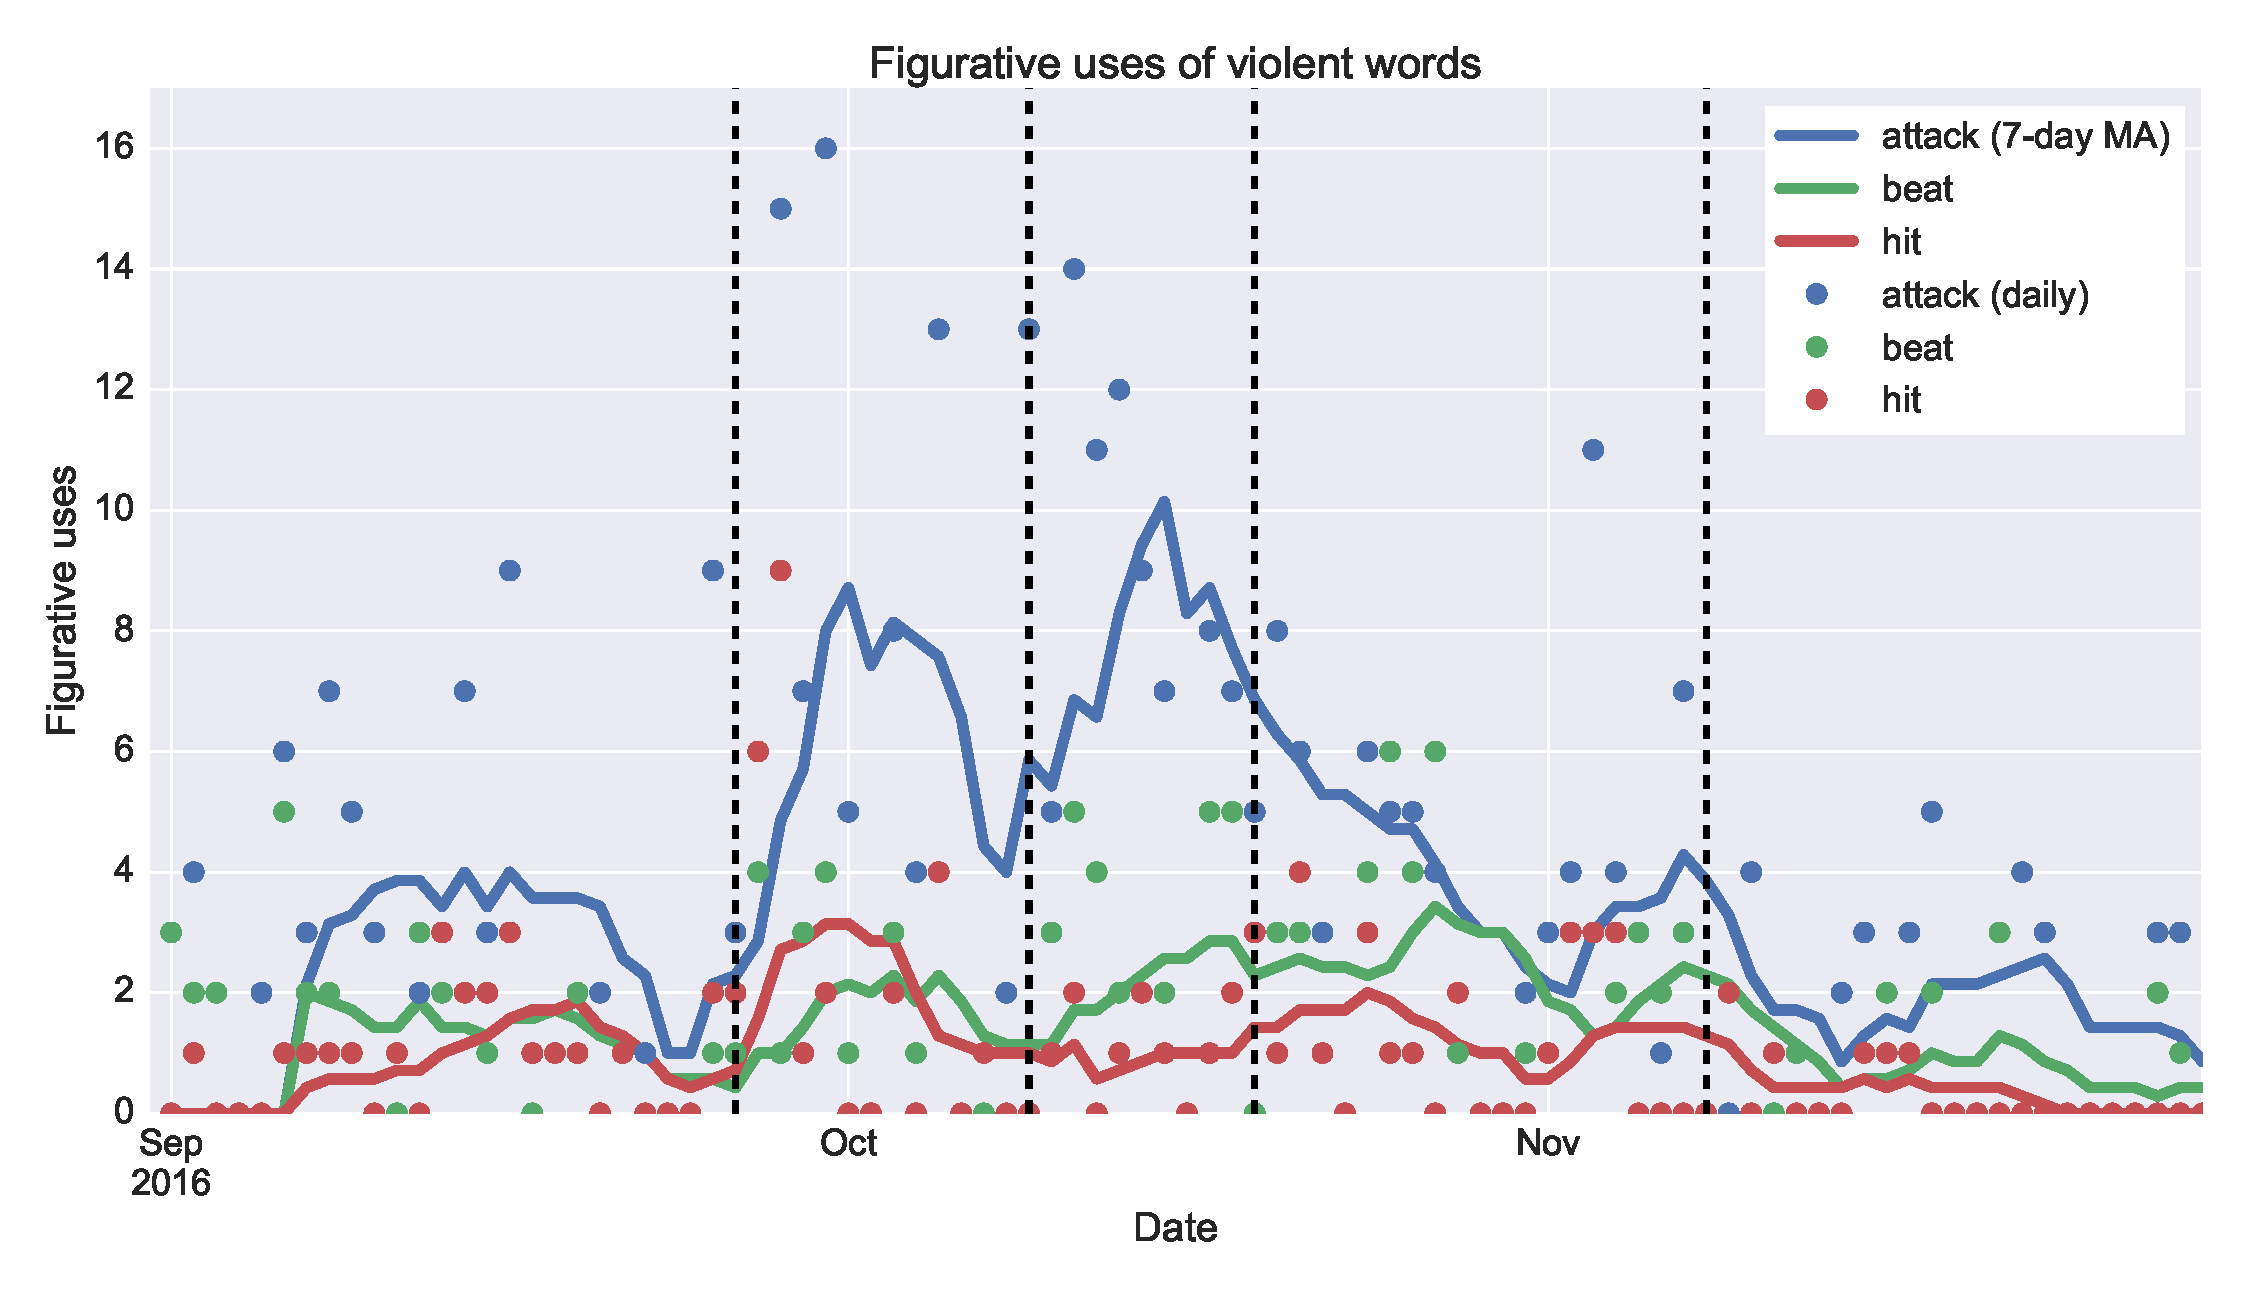
\includegraphics[width=1.25\textwidth]{figures/fig_uses_violent_words-FIG1.pdf}
\end{center}
\caption{
  7-day moving average and daily counts of the figurative uses of the three-most
  used violent words in figurative constructions. Uses come from a variety of
  conceptual metaphors which more or less reduce to 
  \textsc{politics is a physical fight}. The first three dashed 
  vertical lines are the dates of the presidential debates, 
  September 26, October 9, and October 19, 2016. The last dashed
  line is election day, November 8, 2016.
}
\label{fig:timeseries}
\end{figure*}

We want to see if indeed we can identify ``phase shifts'' in figurative 
violence use. The daily usage of the three most common violent words used in 
figurative constructions is shwon in Figure \ref{fig:timeseries}. As discussed more thoroughly in the following sections, we fit a mixed model to the data. We
augment the data with a ``phase'', which is a value of either 1, 2, or 3 if
the date of the count is in either the first, second, or third grouping of 
dates. By varying the start and end date of the second phase and fitting a
model to each start and end date pair, we are able to select the best 
candidates for the dates where phase transitions occur. The first phase 
corresponds roughly to the pre-debate phase, the second phase corresponds to
the debate phase, and the third phase represents post-debate or possibly 
post-debate and post-election. We will show that the first phase transition
seems to happen well past the first debate while the second phase transition
is more fuzzy, but if one date were to be specified, it actually is 
election day itself, November 8, 2016.


